% Tabela: Configurações descartadas no experimento Delta
\begin{table}[H]
	\centering
	\caption{Configurações descartadas de análises pelo Experimento 1.}
	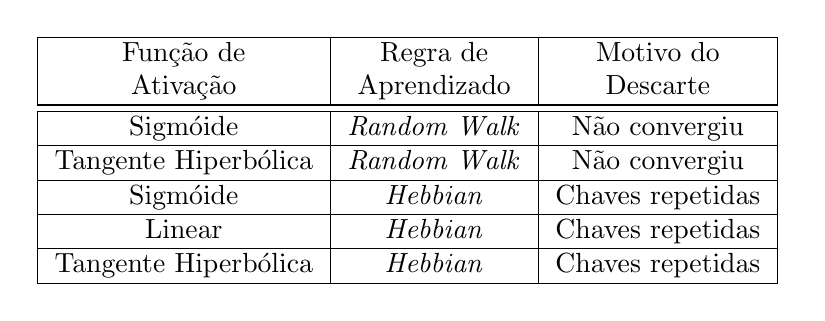
\begin{tikzpicture}

		\node[thick, align=center] (table) {
			\begin{tabular}{ |c|c|c| }
				\hline
				% \multicolumn{3}{ |c| }{Configurações descartadas nas análises} \\
				% \hline \hline
				Função de & Regra de & Motivo do\\
				Ativação & Aprendizado & Descarte\\
				\hline \hline
				Sigmóide              & \textit{Random Walk} & Não convergiu    \\ \hline
				Tangente Hiperbólica & \textit{Random Walk} & Não convergiu    \\ \hline
				Sigmóide              & \textit{Hebbian}     & Chaves repetidas \\ \hline
				Linear               & \textit{Hebbian}     & Chaves repetidas \\ \hline
				Tangente Hiperbólica & \textit{Hebbian}     & Chaves repetidas \\ \hline
			\end{tabular}
		};

	\end{tikzpicture}
% 	\caption{Configurações descartadas de análises pelo Experimento 1.}
	\label{tab:configuracoesDescartadasDelta}
\end{table}